

\section{First ETH3D run (fixed split)}\label{sec:eth3d1}
This experiment removes the two main gaps of the synthetic and Notre Dame experiments of the main paper: the relative rotations and their uncertainty come from a learned network run on real images, and the degradations act on pixels, not on rotations.

\paragraph{Protocol} We use the 13 scenes of the ETH3D high-resolution multi-view training set~\cite{schops2017eth3d}, split by scene before any result was seen: 6 scenes for calibration (electro, kicker, meadow, pipes, relief\_2, terrains) and 7 for testing (courtyard, delivery\_area, facade, office, playground, relief, terrace), so calibration and test share no image and no place. Each sub-scene is a random set of 12 images; the view graph links each image to its 6 nearest cameras by viewing direction and position (on average 38.6 edges). VGGT-1B~\cite{wang2025vggt} is run on every image pair (inputs downscaled to at most 1024\,px, then to VGGT's 518\,px), and the relative rotation is read from its camera head. The edge uncertainty is pre-registered as $\hat\sigma_{ij}=1/\mathrm{median}$ of VGGT's depth confidence over both images. Calibration uses 144 clean sub-scenes (24 per scene; 140 go to the four splits, reshuffled for each of 5 seeds). Each test scene has 10 sub-scenes under 7 conditions: clean; fog rendered with the atmospheric scattering model at median transmission $t\in\{0.7,0.5,0.3\}$, using depth predicted by VGGT on the clean image; low light (Poisson--Gaussian noise at $0.3$ and $0.15$ of the linear exposure); and synthetic rain streaks (490 test graphs). Sub-scenes with a disconnected view graph (4 of 70 per condition) are reduced to their largest component for every method. Edges with error above $5^\circ$ count as outliers; they are 22.4\% of clean test edges and 24--29\% under degradation, and 14--19\% of edges exceed $30^\circ$. Methods, configuration and metrics are those of Section~\ref{sec:protocol} of the main paper; ConfW now uses VGGT's confidence. Seeds only reshuffle the calibration splits, so the unit of inference is the test scene: we average over seeds and sub-scenes per scene and use an exact sign-flip test over the 7 scenes (smallest two-sided $p=1/64$).

\begin{table*}[!htbp]\centering\footnotesize
\caption{ETH3D with the VGGT front end: AUC@5$^\circ$ (mean over the 7 held-out test scenes, 95\% bootstrap interval over scenes; 70 sub-scenes of 12 cameras per condition, 5 calibration seeds). Best mean per row in bold. The last column counts test scenes on which CARA beats CG.}\label{tab:eth3d}
\setlength{\tabcolsep}{3pt}\resizebox{\textwidth}{!}{\begin{tabular}{lcccccccc}\toprule
Condition & CG & ConfW & GLOMAP-RA & Shonan-H & CG-$\hat\rho$ & CARA-static & CARA & CARA$>$CG \\\midrule
clean & 0.621\,{\scriptsize[0.501,0.731]} & 0.654\,{\scriptsize[0.538,0.757]} & 0.626\,{\scriptsize[0.513,0.738]} & 0.589\,{\scriptsize[0.465,0.701]} & 0.628\,{\scriptsize[0.504,0.739]} & \textbf{0.657\,{\scriptsize[0.558,0.735]}} & 0.648\,{\scriptsize[0.538,0.736]} & 3/7 \\
fog $t{=}0.7$ & 0.609\,{\scriptsize[0.484,0.726]} & \textbf{0.640\,{\scriptsize[0.509,0.759]}} & 0.612\,{\scriptsize[0.491,0.729]} & 0.571\,{\scriptsize[0.453,0.687]} & 0.608\,{\scriptsize[0.475,0.730]} & 0.626\,{\scriptsize[0.499,0.736]} & 0.622\,{\scriptsize[0.496,0.733]} & 3/7 \\
fog $t{=}0.5$ & 0.596\,{\scriptsize[0.470,0.716]} & \textbf{0.653\,{\scriptsize[0.533,0.757]}} & 0.594\,{\scriptsize[0.463,0.717]} & 0.545\,{\scriptsize[0.412,0.671]} & 0.593\,{\scriptsize[0.465,0.716]} & 0.618\,{\scriptsize[0.503,0.722]} & 0.613\,{\scriptsize[0.500,0.722]} & 4/7 \\
fog $t{=}0.3$ & 0.569\,{\scriptsize[0.423,0.703]} & \textbf{0.601\,{\scriptsize[0.435,0.739]}} & 0.553\,{\scriptsize[0.389,0.702]} & 0.523\,{\scriptsize[0.372,0.661]} & 0.572\,{\scriptsize[0.435,0.700]} & 0.580\,{\scriptsize[0.449,0.694]} & 0.574\,{\scriptsize[0.427,0.701]} & 4/7 \\
low light $0.3$ & 0.544\,{\scriptsize[0.404,0.677]} & 0.565\,{\scriptsize[0.417,0.706]} & 0.564\,{\scriptsize[0.434,0.682]} & 0.536\,{\scriptsize[0.416,0.659]} & 0.570\,{\scriptsize[0.438,0.692]} & \textbf{0.581\,{\scriptsize[0.444,0.702]}} & 0.565\,{\scriptsize[0.412,0.697]} & 3/7 \\
low light $0.15$ & 0.502\,{\scriptsize[0.355,0.656]} & 0.546\,{\scriptsize[0.387,0.686]} & 0.526\,{\scriptsize[0.395,0.657]} & 0.491\,{\scriptsize[0.350,0.625]} & 0.497\,{\scriptsize[0.353,0.645]} & \textbf{0.584\,{\scriptsize[0.458,0.697]}} & 0.571\,{\scriptsize[0.441,0.689]} & 6/7 \\
rain & 0.528\,{\scriptsize[0.427,0.629]} & 0.524\,{\scriptsize[0.422,0.634]} & 0.512\,{\scriptsize[0.411,0.625]} & 0.505\,{\scriptsize[0.408,0.613]} & 0.528\,{\scriptsize[0.422,0.633]} & 0.534\,{\scriptsize[0.427,0.635]} & \textbf{0.546\,{\scriptsize[0.444,0.646]}} & 3/7 \\
\bottomrule\end{tabular}}\end{table*}


\paragraph{What the degradations do to VGGT} VGGT is robust to these degradations. From clean to the strongest fog and low light, the median error of inlier edges grows only from $0.70^\circ$ to $0.75^\circ$ and $0.85^\circ$ (rain: $1.32^\circ$), while the fraction of edges above $30^\circ$ grows from 14.1\% to 16.7\% and 19.2\%. The shift is therefore mainly more gross failures, not a rescaling of inlier noise, which is the case Assumption~\ref{ass:scale} of the main paper does not cover.

\paragraph{Accuracy} \Cref{tab:eth3d} and \cref{fig:eth3d}(a) report AUC@5$^\circ$. CARA's mean is above CG, GLOMAP-RA and Shonan-H in all seven conditions (by $0.005$--$0.069$ over CG, largest under low light at $0.15$), but the per-scene intervals overlap and CARA beats CG on only 3 to 6 of the 7 test scenes depending on the condition. Pooled over conditions the difference to CG is $+0.024$ (3 of 7 scenes, $p=0.47$) and to GLOMAP-RA $+0.022$ ($p=0.50$); only Shonan-H is beaten consistently (6 of 7 scenes, $p=0.047$, Holm-adjusted $0.23$). None of these differences is significant. ConfW, which only weights CG by VGGT's confidence, is as accurate as CARA (pooled difference $-0.006$) and has the lowest catastrophic rate in four of seven conditions; CARA's gates reject 60--80\% of outlier edges but also 8--10\% of inliers, and on 12-camera graphs this removes support that weighting keeps. CARA-static is within $0.016$ of CARA in every condition and slightly higher in six of seven, so the drift factor does not improve accuracy here, as expected when the inlier noise barely changes.

\begin{table}[!htbp]\centering\footnotesize
\caption{ETH3D with VGGT: per-camera bounds at target $1-\alpha_{\mathrm{cam}}=0.9$ (mean over test scenes, 95\% interval over scenes), median $\hat\rho$, and the ratio of the median inlier edge error to its clean value.}\label{tab:eth3dbounds}
\setlength{\tabcolsep}{2.5pt}\begin{adjustbox}{max width=\textwidth}\begin{tabular}{lcccccc}\toprule
 & \multicolumn{2}{c}{CARA} & \multicolumn{2}{c}{CARA-static} & & \\\cmidrule(lr){2-3}\cmidrule(lr){4-5}
Condition & cov. & hard & cov. & hard & $\hat\rho$ & ratio \\\midrule
clean & 0.886 & 0.760 & 0.887 & 0.774 & 1.00 & 1.00 \\
fog $t{=}0.7$ & 0.843 & 0.721 & 0.827 & 0.710 & 1.13 & 0.97 \\
fog $t{=}0.5$ & 0.841 & 0.737 & 0.832 & 0.751 & 1.11 & 0.99 \\
fog $t{=}0.3$ & 0.789 & 0.681 & 0.800 & 0.690 & 1.37 & 1.07 \\
low light $0.3$ & 0.812 & 0.691 & 0.813 & 0.709 & 1.24 & 1.13 \\
low light $0.15$ & 0.823 & 0.698 & 0.806 & 0.691 & 1.44 & 1.21 \\
rain & 0.852 & 0.717 & 0.810 & 0.678 & 1.42 & 1.89 \\
\bottomrule\end{tabular}\end{adjustbox}\end{table}


\paragraph{Per-camera bounds} On clean held-out scenes the calibrated bounds cover 88.6\% of registered cameras (95\% interval $[82.2,94.5]$\%) at a 90\% target (\cref{tab:eth3dbounds}, \cref{fig:eth3d}(b)). This is the first test of the guarantee with a learned front end, calibration and test on different places, and a real uncertainty proxy, and the result is consistent with the target. Under degradation, coverage falls to 78.9--85.2\%, and to 68--74\% on the quarter of cameras with the largest $u_i$. The drift factor responds ($\hat\rho$ median $1.1$--$1.4$ under shift, $1.0$ on clean scenes) and raises coverage over CARA-static by 1--4 points under rain ($85.2$ vs $81.0$\%), fog $0.7$, fog $0.5$ and low light $0.15$, but not under fog $0.3$ or low light $0.3$. A scalar noise factor cannot account for a higher rate of gross failures, so these bounds are optimistic by about 5--11 points under real shift.

\begin{figure}[!htbp]\centering
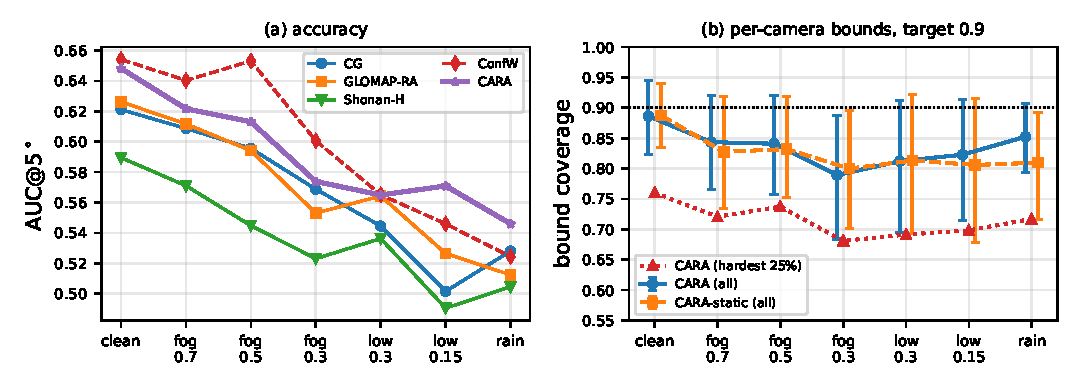
\includegraphics[width=\columnwidth]{figs/eth3d.pdf}
\caption{ETH3D with VGGT. (a) AUC@5$^\circ$ per condition (mean over 7 test scenes). (b) Coverage of the 90\% per-camera bounds with 95\% intervals over test scenes, and coverage on the hardest quarter of cameras; dotted line: target.}\label{fig:eth3d}
\end{figure}

\paragraph{Choice of confidence aggregate} VGGT's depth confidence has a floor of $1$, and for 55\% of edges the median over both images sits on it, so the pre-registered $\hat\sigma$ is constant on most edges. The pre-registered alternative, the exponential of the negative mean log-confidence, separates outlier edges much better (AUROC $0.89$ vs $0.73$ on clean test edges; Spearman correlation with error $-0.69$ vs $-0.44$). With it CARA's AUC@5 rises by $0.01$ on average ($0$ to $0.018$ per condition) (pooled difference to CG $+0.035$, 4 of 7 scenes, $p=0.36$), ConfW rises as well, and the coverage pattern is unchanged (CARA 88.8\% clean, 79.8--85.5\% under shift). We report the pre-registered aggregate in the tables.
